\subsection{The 256-group baseline screen}\label{app:screen256}
\begin{figure*}[!tp]
\centering

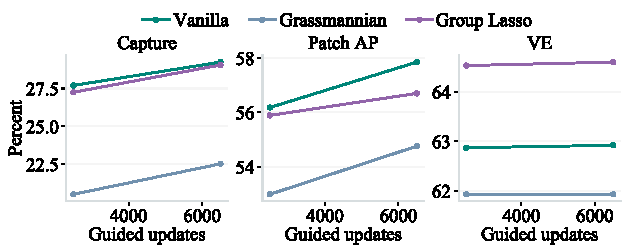
\includegraphics[width=287.28bp]{figures/agf_plot_screenextended.pdf}
\caption{Extended 256-group screen. Guided training budget is listed explicitly. Neither row is an independent confirmation.}
\label{tab:screenextended}

\end{figure*}

\paragraph{Why Vanilla is the base architecture.}
Capture directly addresses our research question by measuring the object
contrast reconstructed by one group. In the initial COCO screen,
Vanilla has the highest native Capture at 21.31\%, versus 16.84\% for
Grassmannian and 20.47\% for Group Lasso
(Table~\ref{tab:released-screen-detail}). With GGF training,
Vanilla also has the highest Capture and Patch AP at 27.70\% and 56.18\%.
Grassmannian reaches 20.52\% and 52.99\%, and Group Lasso reaches
27.25\% and 55.89\%. These initial object-alignment results motivate
developing GGF on the Vanilla architecture.

Additional studies support the choice. On Manifold Zoo, Vanilla leads
the unsupervised variants in both single-group factor recovery and full
reconstruction (Table~\ref{tab:synthetic-means}). Recovery is
$96.781\pm0.533$\%, versus $86.782\pm0.776$\% for Grassmannian and
$93.295\pm1.548$\% for Group Lasso. Reconstruction VE is
$97.372\pm0.043$\%, versus $92.049\pm0.183$\% and $96.694\pm0.131$\%.
In the 1,024-group COCO controls, Vanilla has the highest mean VE
and higher mean Patch AP than Group Lasso
(Table~\ref{tab:matched-seed-scores}). Grassmannian has higher Patch AP,
and Group Lasso has slightly higher Capture in that comparison.
The choice therefore follows the initial Capture result and supporting
recovery and reconstruction evidence, while retaining the metric tradeoffs observed at 1,024 groups.

\begin{agfresulttable}
\caption{The 256-group baseline screen on 800 test images, seed 1. Scores are percentages.}\label{tab:released-screen-detail}
\begin{tabular}{@{}llrrr@{}}
\toprule
Class & State & Capture & AP & VE \\
\midrule
Vanilla & Native & 21.31 & 50.74 & 63.48 \\
Vanilla & GGF & 27.70 & 56.18 & 62.87 \\
Grassmannian & Native & 16.84 & 51.78 & 62.09 \\
Grassmannian & GGF & 20.52 & 52.99 & 61.93 \\
Group Lasso & Native & 20.47 & 52.45 & 65.24 \\
Group Lasso & GGF & 27.25 & 55.89 & 64.53 \\
\bottomrule
\end{tabular}

\end{agfresulttable}

The 256-group screen trains for 40 epochs at each maximum learning rate
(0.0004, 0.003) and selects the minimum-MSE checkpoint. Group Lasso also
requires activity in the range 12.8--19.2 (20\% tolerance). Its measured 18.50
passes this check but differs from Top-16. Both arms of the scaled comparison
use Vanilla.

The fixed-group guided screen uses 1,500 updates plus two 500-update segments, resetting Adam between segments. Its search-budget control receives 6,500 guided updates. Scaled confirmation instead keeps continuous Adam in both 2,500-update arms. These budgets are distinct and do not establish optimal native training duration.

\subsection{Three-direction supervised pilot controls}\label{app:maskinit}\label{app:pending}\label{app:slics-results}
The three-direction SLiCS pilots used 75 groups of three directions, a Top-16
inference sensitivity, shorter training, and the inspected test cohort.
They examined mask versus image-label support and native versus mask-derived
GGF initialization. Finite-solver nonconvergence and different checkpoint
rules limit those comparisons. They are not pooled with the completed
twelve-direction study in Appendix~\ref{app:supervised-five}, which retains
all retained trained endpoints, independently defined partial-concept readouts,
and strict full-dictionary reconstruction checks. The pilot numerical
records, solver failures and protocol are preserved in the repository,
including \path{evidence/supervised_five_seed/historical_slics_details.tex}.
